\section{Summary of Paper \ref{pap:vct}}
\subsection*{"\nameref{pap:vct}"}
\subsection*{Scope and motivations}
The objective of paper \ref{pap:vct} was to propose a parametric model structure based on physical insights from VCT and FT inverse dynamics. The reference model from Paper \ref{pap:physics} was assumed to be close to the physically correct true model of ship manoeuvring dynamics. This model was developed with VCT, which is based on physical first principles through CFD calculations. Paper \ref{pap:vct} investigated the identification of manoeuvring with VCT more closely, with the aim of achieving a model that more accurately reflected the true system.

Manoeuvring models were developed for the two WAPS test cases with large rudders. The models were identified by conducting a VCT to obtain hydrodynamic damping coefficients and by conducting pure yaw and pure sway tests in FNPF to obtain the added masses using the Fourier series method (see \autoref{sec:fourier}). The identified force models were compared with the inverse dynamics forces of the zigzag tests to identify potential weaknesses within the models.

\subsection*{Results and main findings}
Propeller and rudder forces were measured during the FRMTs for Optiwise. It was found that these measured forces together with forces predicted with a hull sub module, identified from VCT data, could recreate the estimated inverse dynamics forces during zigzag maneuvers with sufficient accuracy. Much effort was therefore devoted to finding a rudder force prediction model that could recreate the rudder forces for Optiwise. A modified quadratic MMG rudder model was proposed (see \autoref{sec:MMG_rudder}) as an improved version of the original model \cite{yasukawaIntroductionMMGStandard2015}. 
\autoref{fig:MMG_quadratic} shows the Optiwise rudder force $Y_R$ for the various VCT test types (see \autoref{sec:VCT}) plotted against the effective rudder angle $\beta_R$. The original MMG rudder model has a constant flow straightening factor $\gamma_{Rpos}$ for positive $\beta_R$ and another constant flow straightening factor $\gamma_{Rneg}$ for negative $\beta_R$. The proposed quadratic formulation has two additional parameters, $\gamma_{R2pos}$ and $\gamma_{R2neg}$, that allow the flow straightening to vary with $\beta_R$ that better fits the VCT data.
\begin{figure}[h]
     \centering
     \begin{subfigure}[b]{0.49\textwidth}
         \centering
         \includesvg[width=1\textwidth]{figures/results_optiwise_VCT.Y_R_MMG_original.svg}
        \caption{Original MMG rudder model.}
        \label{fig:Y_R_MMG_original}
     \end{subfigure}
     \hfill
     \begin{subfigure}[b]{0.49\textwidth}
         \centering
         \includesvg[width=1\textwidth]{figures/results_optiwise_VCT.Y_R_MMG_quadratic.svg}
        \caption{Modified quadratic MMG rudder model.}
        \label{fig:Y_R_MMG_quadratic}
     \end{subfigure}
    \caption{Rudder force during the VCT tests as a function of the effective inflow angle for the original MMG model and the modified quadratic MMG model.}
    \label{fig:MMG_quadratic}
\end{figure}

The rudder forces during the Optiwise FRMTs were predicted and compared with the corresponding measured forces, as shown in \autoref{fig:rudder_forces}. Although there were some minor deviations during the zigzag10/10 test, there was generally good agreement between the predictions and measurements. VCT calculations of some of the states during the manoeuvres have also been added to this comparison, which also show good agreement.
\begin{figure}[h]
    \centering
    \begin{subfigure}[b]{\textwidth}
        \centering
        \includesvg{figures/results_optiwise_ID.rudder_forces_zigzag 10_10.svg}
        \caption{Zigzag10/10 to port.}
        \label{fig:ID_measured_rudder_zigzag_10_10}
    \end{subfigure}
     \vfill
    \begin{subfigure}[b]{\textwidth}
        \centering
        \includesvg{figures/results_optiwise_ID.rudder_forces_zigzag 20_20.svg}
        \caption{Zigzag20/20 to starboard.}
        \label{fig:ID_measured_rudder_zigzag_20_20}
    \end{subfigure}
    \caption{Rudder forces during the zigzag tests compared to predictions with the MMG models.}
    \label{fig:rudder_forces}
\end{figure}

The total forces during the zigzag tests were also predicted, including the hull and rudder models. \autoref{fig:ID_optiwise20}  shows a comparison between the predicted forces and FRMT inverse dynamics forces. VCT calculations of some of the states during the manoeuvres have also been added to this figure, which agrees well with the model predictions.
However, deviations were observed for the sway force $Y_D$ within three seconds after the rudder changes at t = 11--14 s and t = 35--38 s, for the zigzag10/10 and t = 11--14 s, t = 35--38 s, t = 64 s, for the zigzag20/20. The model and state VCT calculations predict a straighter line in the $Y_D$ time series near these deviation points. No reasonable explanation for these deviations has been found, and filtration errors in the EKF were ruled out as a possible explanation.
\begin{figure}[h]
    \centering
    \begin{subfigure}[b]{\textwidth}
        \centering
        \includesvg{figures/results_optiwise_ID.zigzag 10_10.svg}
        \caption{Zigzag10/10 to port.}
        \label{fig:ID_MMG_zigzag_10_10}
    \end{subfigure}
     \vfill
    \begin{subfigure}[b]{\textwidth}
        \centering
        \includesvg{figures/results_optiwise_ID.zigzag 20_20.svg}
        \caption{Zigzag20/20 to starboard.}
        \label{fig:ID_MMG_zigzag_20_20}
    \end{subfigure}
    \caption{Inverse dynamics forces during the zigzag tests compared to predictions with the MMG models.}
    \label{fig:ID_optiwise20}
\end{figure}

Closed loop simulations were also conducted, as shown in \autoref{fig:sim_optiwise}, and exhibited strong agreement for the zigzag20/20 tests and a slightly lower agreement for the zigzag10/10 tests.
It can therefore be concluded for the Optiwise case that
the VCT data contained correct damping forces during the maneuvers, which were well
described by the chosen model structure, including the proposed rudder model, and that the method used to determine added masses produced reasonable values.
\begin{figure}[h]
     \centering
     \begin{subfigure}[b]{0.49\textwidth}
         \centering
         \includesvg{figures/results_optiwise_ID.closed loop zigzag 10_10 port.svg}
         %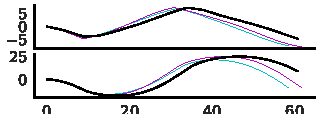
\includegraphics[]{figures/results_optiwise_ID.closed loop zigzag 10_10 port.pdf}
        \caption{Zigzag10/10 to port.}
        \label{fig:sim_optiwise_10_port}
     \end{subfigure}
     \hfill
     \begin{subfigure}[b]{0.49\textwidth}
         \includesvg{figures/results_optiwise_ID.closed loop zigzag 10_10 stbd.svg}
         %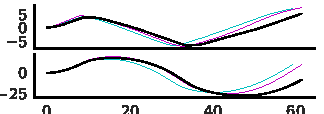
\includegraphics[]{figures/results_optiwise_ID.closed loop zigzag 10_10 stbd.pdf}
        \caption{Zigzag10/10 to starboard.}
        \label{fig:sim_optiwise_10_stbd}
     \end{subfigure}
     \vfill
     \begin{subfigure}[b]{0.49\textwidth}
         \centering
         \includesvg{figures/results_optiwise_ID.closed loop zigzag 20_20 port.svg}
         %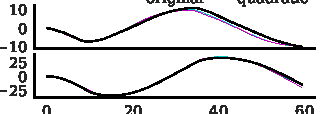
\includegraphics[]{figures/results_optiwise_ID.closed loop zigzag 20_20 port.pdf}
        \caption{Zigzag20/20 to port.}
        \label{fig:sim_optiwise_20_port}
     \end{subfigure}
     \hfill
     \begin{subfigure}[b]{0.49\textwidth}
         \includesvg{figures/results_optiwise_ID.closed loop zigzag 20_20 stbd.svg}
         %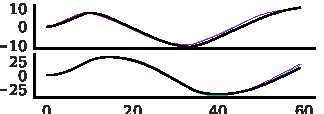
\includegraphics[]{figures/results_optiwise_ID.closed loop zigzag 20_20 stbd.pdf}
        \caption{Zigzag20/20 to starboard.}
        \label{fig:sim_optiwise_20_stbd}
     \end{subfigure}
     
        \caption{Comparison of zigzag tests between Optiwise experiments (black) and simulations with the MMG original (cyan) and MMG quadratic (purple).}
        \label{fig:sim_optiwise}
\end{figure}